% 1. in union-find subsection make function names in text a different
%    font
% 2. include parameters of size-constrained add-edge on randomized graph
%    in table
% 3. more analysis of SC AE results
%#######################################################################

We introduce several algorithms for generating brain parcellations. The
algorithms in this chapter are all local search heuristics; they begin
with $n$ unconnected vertices and iteratively join adjacent ones into
components until some stopping criterion is met.

For each algorithm, the resulting parcellation is presented, discussed,
and evaluated according to the criteria introduced in the previous
chapter.

\section{The Add-Edge Algorithm}

The first and simplest algorithm starts with an empty graph of $n$
vertices and sequentially adds edges between adjacent voxels in order of
highest sample distance correlation, until the graph has some
prespecified number of connected components $k$. We will refer to this
algorithm as ``Unconstrained Add-Edge''.

The Unconstrained Add-Edge algorithm produces severely imbalanced
parcellations. In the 100-component graph, there was one component
containing over 99.9\% of all the vertices in the graph.

Our attempt to address this problem was to impose a filter on each edge
considered, adding the edge only if at least one of the two following
conditions are met:

\begin{enumerate}[1.]
\item
At least one of the two components bridge by the edge is of size less
than some prespecified parameter $s_{\min}$.

\item
The union of the two components is of size $\leq s_{\max}$.
\end{enumerate}

The restriction on adding new edges was not successful in creating
balanced partitions.

\subsection{Implementation of Unconstrained Version}

A naive implementation of Unconstrained Add-Edge would re-compute the
number of connected components in the graph (using linear-time
bread-first or depth-first search) after each addition of an edge,
resulting in a costly $O(EN)$ time complexity. A more efficient
implementation takes advantage of the fact that each addition of an
edge decreases the number of components in the graph by at most 1.
Hence the algorithm needs only to compute the number of connected
components after adding $c - k$ edges, where $c$ is the current number
of connected components of the graph, beginning at $n$.

Another implementation uses a binary search-type strategy and is
$O((n + E) \log E)$. The idea is to ``search'' for the last edge to add
to the graph by maintaining a range of possible last edges. In each
iteration, the algorithm would add to the graph edges 1 to the midpoint
of this range, compute the number of connected components, and adjust
the range based on whether the number of components is higher or lower
than the target $K$.

\subsection{Implementation of Size-Constrained Version using Union-Find}

The naive implementation must use BFS/DFS in each iteration to compute
the sizes of the two components to be connected by an edge, and hence
must have time complexity $O(EN)$. Fortunately, there is a way to
sublinearly update information on the components of the graph, using
the union-find data structure.

The core Union-Find data structure begins with an empty graph of $N$
vertices and supports two operations. union(i, j) adds an edge between
vertices $i$ and $j$. root(i) returns an identifier for the component
to which vertex $i$ belongs. All vertices in the same component have the
same root. We modified Union-Find to support an additional operation.
component\_size(i) returns the number of vertices belonging to the
component containing $i$.

Union-Find represents each component as a rooted tree, with vertices in
the graph mapping to nodes in the tree. Information about the tree is
stored in two arrays of length $N$, parent and size, which are subject
to the following invariants.

\begin{enumerate}[1.]
\item
For each node i, parent[i] = node i's parent on the tree, unless i is a
root node. If i is a root node, then parent[i] = i.

\item
Nodes i and j are in the same component if and only if they are in the
same tree, if and only if they share the same root node.

\item
If i is a root node, then size[i] = the size of the component, or the
number of nodes in the tree. If i is not a root node, then size[i] can
be anything.
\end{enumerate}

A baseline implementation of the three functions is

\begin{algorithm}
\caption{Union-Find}
\begin{algorithmic}

\Function{root}{i}
    \While{parent[i] $\neq$ i}
        \State i $\gets$ parent[i]
    \EndWhile
    \State \Return i
\EndFunction
\State 

\Function{union}{i, j}
    \State parent[root(j)] $\gets$ root(i)
\EndFunction
\State 

\Function{component\_size}{i}
    \State \Return size[root(i)]
\EndFunction

\end{algorithmic}
\end{algorithm}

In addition to the baseline code above, there are two important
optimizations:

\begin{enumerate}[1.]
\item
Weighted union maintains information of the sizes of each component so
that the root of the smaller component always becomes a child of the
larger component's root.

\item
Path compression flattens the tree with each call to root. Specifically,
when root is called on node $i$, each node traversed from $i$ to the
root has its parent set to be the root.
\end{enumerate}

With these two optimizations, the time complexity of root, union, and
component\_size has been shown to be at least as good as $O(\log^* N)$
where $\log^*$ is the iterated logarithm, defined as the number of
times the natural log must be applied to $N$ so that it becomes less
than or equal to 1.

\section{The Edge-Contraction Algorithm and Contractible Graphs}

We propose a new data structure called the \textit{Contractible Graph}
(CG) for brain parcellation. The rationale behind the CG is a heuristic
procedure for partitioning a graph into somewhat balanced components
so as to maximize the Adjacent-Score (\ref{adjacent-score}).

The CG is a mapping of the vertices of the original graph to the
vertices of a new graph. The vertices of the CG are called
\textit{components} and between any two components there exists exactly
one weighted edge, henceforth called a \textit{link}. The weight
of a link $w_{A,B}$ between two components $A$ and $B$ in the CG equals
the average weight of all edges in the original graph between vertices
mapped to $A$ and vertices mapped to $B$. If no such edges exist,
the weight of the link is $0$. Formally,

\[ E_{A,B} = \{(i, j) \in E : i \in A, j \in B\} \]
\[ w_{A,B} = \begin{cases}
    \frac{1}{|E_{A,B}|} \sum_{(i,j) \in E_{A,B}} w_{ij} &
        \text{if } |E_{A,B}| > 0 \\
    0 & \text{otherwise}
\end{cases} \]

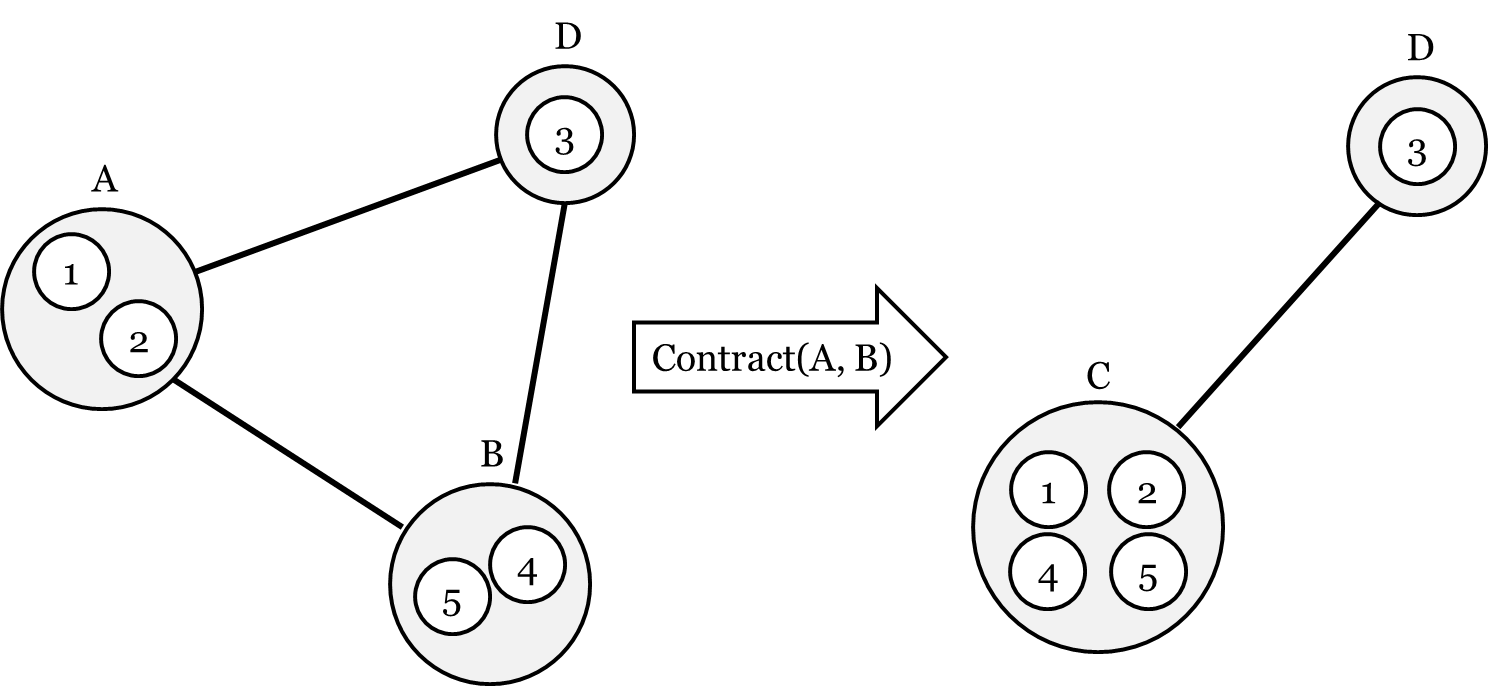
\includegraphics[scale = 0.55]{figs/4_contractible_graph}

We say an edge $(i,j)$ is \textit{between} components $A$ and $B$ if
$i$ is in one of $A$ or $B$ and $j$ is in the other. The \textit{size}
of a component is the number of vertices it contains.
A \textit{contraction} of a link $(A,B)$ in a CG replaces components
$A$ and $B$ with a new component (call it $C$) containing all vertices
mapped to $A$ or $B$, as illustrated in the figure above.
Component $C$ has one link to every other component in the CG, whose
weights are the mean of the weights of the corresponding vertex edges,
or $0$ if no edge exists. Thus the contraction operation maintains the
link-invariant property of CG. This leads to the Edge-Contraction
algorithm, which begins with the original graph with all vertices as
singleton components and contracts edges in a certain order until the
graph has only $k$ components in all.

\begin{algorithm}
\caption{Edge-Contraction}
\begin{algorithmic}
\State \textbf{Input:} Undirected positive-weighted graph $G$ and
       target component number $k$
\State Create a CG from $G$ so that every vertex maps to
       a unique component
\Repeat
\State $\mathcal{S} \gets$ smallest component(s) in the CG
\State $(A,B) \gets \argmax{A \in \mathcal{S}} w(A,B)$
\State Contract $(A,B)$
\Until{CG has $k$ components}
\State \textbf{Output:} Components of CG
\end{algorithmic}
\end{algorithm}

Why does Edge-Contraction work better than the previous algorithms?
The Edge-Contraction algorithm attempts to address two problems of
the Size-Constrained Add-Edge algorithm: unbalanced parcels and poor
Adjacent-Score relative to randomized graph. It solves the former
problem by prioritizing edges that are connected to small components.

The low Adjacent-Score is likely due to the following scenario:
when a vertex is added to a component, it might have multiple
edges to that component. One edge might have a very high weight; this is
the one that is officially ``added''. However, the other edges with far
lower weights are implicitly added as well, lowering the average edge
weights within the component.

The Edge-Contraction algorithm handles this issue by maintaining that
there can be at most one edge between any two components A and B, and
further that the weight on such an edge is the mean of the weights on
all edges that connect a vertex in A with a vertex in B.

\subsection{Implementation using Nested Hash Tables and Priority Queue}

In a Contractible Graph, the weight of the link between two components
depends on the summed weight of all edges between them, and the number
of such edges.

Our implementation of the CG uses \textit{nested hash tables},
diagrammed below. The outer hash table maps each component $A$ to an
inner hash table, which maps all components $B$ with a positive link to
$A$ to 1) the summed weights of the edges and 2) the number of edges
between $A$ and $B$.

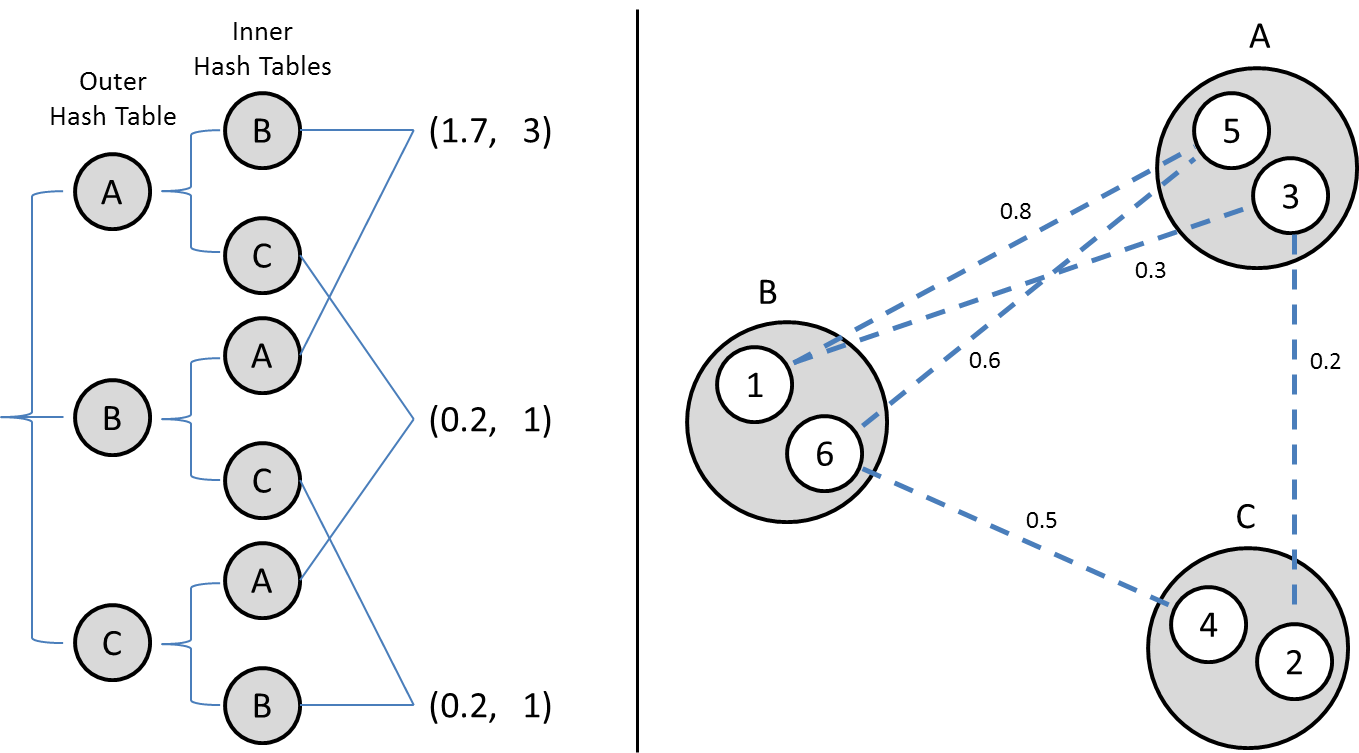
\includegraphics[scale = 0.6]{figs/4_cg_implement}

Implementing the contraction of components $B$ and $C$ into a new
component $D$ on this nested hash table requires the following steps.
The time complexity is stated assuming no hash collisions.

\begin{enumerate}
\item
Compute $\mathcal{X}$, the set of all components that either $B$ or $C$
is linked to. $O(|E_B| + |E_C|)$

\item
Create a new element in the outer hash table, $D$, and associate it
with an empty inner hash table. $O(1)$

\item
For each component $X \in \mathcal{X}$,
\begin{itemize}
\item
Retrieve $W(X,B) + W(X,C)$, the summed weights all edges between $X$
and $B$ and between $X$ and $C$, and $|E_{X,B}| + |E_{X,C}|$, the
number of such edges. These quantities are stored explicitly as a
values in the inner hash table, so this operations is $O(1)$.

\item
Add a new component name $D$ to the inner hash table of $X$ and map it
to $\big( W(X,B) + W(X,C), |E_{X,B}| + |E_{X,C}| \big)$. Delete
elements $B$ and $C$ from the inner list of $X$. $O(1)$

\item
In the $D$ inner hash table, add component name $X$ and map it to
to the same $\big( W(X,B) + W(X,C), |E_{X,B}| + |E_{X,C}| \big)$.
$O(1)$
\end{itemize}

\item
Delete $B$ and $C$ from the outer list.
\end{enumerate}

Having described the contraction step, we will next discuss how to
efficiently locate the link to be contracted.
In computer science, a \textit{Maximum Priority Queue} (MaxPQ) data
type is a set of well-ordered objects that supports the following
operations:

\begin{itemize}
\item
\textit{add(obj)}: Adds an object to the set.

\item
\textit{remove\_maximum()}: Removes and returns an object with the
largest priority in the set.
\end{itemize}

Using the heap data structure, the above two operations both run in
$O(\log n)$ time.

Each component on the CG will be associated with an element of the
priority queue. The priority of component $A$ is defined as
\[ \max_{X}\;w_{A,X} - |A| \]
Since our graph link and edge weights are all between 0 and 1, the
highest priority element in the queue always has the smallest size.
Therefore, if the priority queue is up-to-date with the CG, the
next link to be contracted according to Edge-Contraction has
an endpoint component whose priority is the highest in the queue.

However, a complication arises from the fact that a contraction can
change the priorities of components neighboring the contracting
components, thereby making the priorities stored in the MaxPQ
out-of-date. For instance, if components $A$ and $B$ are contracted, and
there is a component $C$ with positive links to both $A$ and $B$, then
the $C-A$ and $C-B$ links will be replaced by a $C-(AB)$ link with a
different weight. If either $C-A$ or $C-B$ links happened to be the
maximum-weighted links of $C$, then $C$'s priority will be lower,
and $C$ ought to be further down the queue.

To address this issue, we could re-compute the priority of every
component drawn from the MaxPQ. If the component's actual priority is
not the maximum, then it is re-inserted into the queue with updated
priority. Additionally, the maximum priority component may no longer
exist in the CG due to contraction with another component. In this case
it is simply discarded.

Without using an efficient priority queue, the linear searching method
of finding the next link to contract results in a $O\big(n (n-k)\big)$
time algorithm. Using the priority queue the time complexity of
Edge-Contraction is $O \big((n - k) (m + \log n)\big)$, where $m$ is
the average number of positive links a component has.

\subsection{Results}

\begin{table}
\caption{Results of Edge-Contract for Different Component Numbers}
\csvautotabular{figs/4_edge_contract_results.csv}
\label{4_ec}
\end{table}

The Edge-Contract parcellations notably outperformed the anatomical AAL
parcellation in the Adjacency-Score. For further comparison, found the
mean edge weight in the graph to be 0.7258, which is even slightly
higher than the average adjacent within-parcel edge in AAL. This
suggests that the AAL parcellation has no connection with the functional
information contained in this fMRI data set. It shows on the other
hand that the Edge-Contract algorithm can successfully locate regions of
functional similarity.

The one apparent deficiency of Edge-Contract is the jaggedness of its
parcels. Comparison of our parcellations with the AAL shows that our
116-component parcellation -- the same number of components as AAL --
has an average parcel surface area roughly
$\big( \frac{92.14}{29.62} \big)^{\frac{2}{3} }\approx 2.11$ times
that of AAL. Visually, that difference is shown in the plots below of
a typical component from each parcellation.

%\includegraphics[scale = 1]{figs/4_edgecontract_aal_3D}

\section{The Generalized Edge-Contraction Algorithm}

In the original Edge-Contraction algorithm, the criteria for selecting
the next link to contract was to search through the set of smallest
components and find the link of maximal weight. Because this criteria
takes no account of the shape of the two components to be contracted,
the resulting parcels tend to be very jagged.

To address this we expanded the criterion for finding the next link
to contract. Rather than use only the size of the component and the
weight of the link, a \textit{Generalized Edge-Contraction} algorithm
may use any piece of information stored in the Contractible Graph about
a pair of components, such as the number of edges connecting two
components. A \textit{priority function} takes information of any two
components in a CG and outputs a real number, the priority. For each
iteration, the pair of components with the largest priority is
contracted and the priorities of neighboring components with respect
to the newly conjoined component are computed.

For two components $A,B$ let $|A|$ denote size (number of vertices)
of $A$, $E_{A,B}$ denote the set of edges between $A$ and $B$, and
$w_{A,B}$ the weight of the link connecting $A$ and $B$.
The priority function of the original Edge-Contraction algorithm
is $p_0(A, B) = w_{A,B} - |B|$.

\begin{table}
\caption{Results of Generalized Edge-Contract for Various Parameter Settings}
\centering
\begin{subtable}[v]{0.5\textwidth}
  \begin{tabular}{|c|c|c|c|c|}
\hline
$\alpha$ & $\beta$ & Adjacent & Jaggedness & Balance \\
\hline
3 & 1 & 0.7500 & 25.3 & 0.285 \\ 
6 & 1 & 0.7574 & 31.0 & 0.231 \\
10 & 1 & 0.7634 & 36.6 & 0.211 \\
6 & 2 & 0.7565 & 31.0 & 0.199 \\
6 & 4 & 0.7576 & 30.9 & 0.270 \\
\hline
\end{tabular}

  \caption{116 Parcels}
\end{subtable}
~
\begin{subtable}[v]{0.5\textwidth}
  \begin{tabular}{|c|c|c|c|c|}
\hline
$\alpha$ & $\beta$ & Adjacent & Jaggedness & Balance \\
\hline
3 & 1 & 0.7592 & 23.8 & 0.218 \\
6 & 1 & 0.7651 & 28.0 & 0.143 \\
10 & 1 & 0.7705 & 32.0 & 0.221 \\
6 & 2 & 0.7670 & 28.2 & 0.169 \\
6 & 4 & 0.7669 & 28.8 & 0.293 \\
\hline
\end{tabular}

  \caption{300 Parcels}
\end{subtable}
\label{gen_ec}
\end{table}

A link $(A, B)$ will have high priority if either component is small,
if the link has a large weight, and if it has a good boundary-ratio,
defined as $\frac{|E_{A,B}|}{\min(|A|,|B|)}$, which helps to minimize
jaggedness. From these notions we created a family of priority
functions indexed by tunable parameters $\alpha$ and $\beta$
\[ p_1(A, B) = \frac{w_{A,B}^\alpha}{|A|^\beta} \cdot
               \frac{|E_{A,B}|}{\min(|A|,|B|)} \]
that modulate the balance of small size, large weight, and high
boundary ratio. Table \ref{gen_ec} shows the results of the
116-component and 300-component Generalized Edge-Contract parcellation
when performed for various values of $\alpha$ and $\beta$. The adjacent
scores have fallen on average from 0.79 in the vanilla edge contraact
to 0.75 here. This implies a tradeoff between prioritizing edge weight,
jaggedness, and balance in producing a parcellation.

With a balance score of 0.332, the AAL parcellation was better balanced
than all of the parcellations obtained via this priority function,
though not drastically. In terms of jaggedness, these parcellations
all fell within the vicinity of AAL. In this one brain, the best
parcellation arises from parameters $\alpha = 6$ and $\beta = 4$.

Parcellations of other brains using generalized edge contract can be
found in chapter 8.
